\chapter{System Structure}

The system is composed by three types of FMUs: sensor, control and plant.

\begin{description}
	\item Sensor FMUs are four (far left, mid left, mid right, far right),
		everyone corresponds to a different sensor into the line
		follower robot. Sensors produce values from 0 to 255. The value
		0 represents a white line; the value 255 a black line and the
		other values are different tonalities of grey.
	\item The control FMU produces value for the speed of the two wheels,
		having in input values from sensors. For the left wheel values
		are positive and go from 0 to 1; for the right wheel values are
		negative and goes from 0 to -1. The greater is the absolute
		value, the greater is the movement speed. When speeds are equals
		the robot goes straight. If the left speed is below than the
		right one the robot turns left and vice versa.
	\item The plant FMU receives as input the speed values and use it for
		the actuators that realize the command. The robot position (x,
		y, theta) is sent for checks to the four sensors.
\end{description}

\figref{fig:structure} shows the structure of the system.

\begin{figure}[htb]
	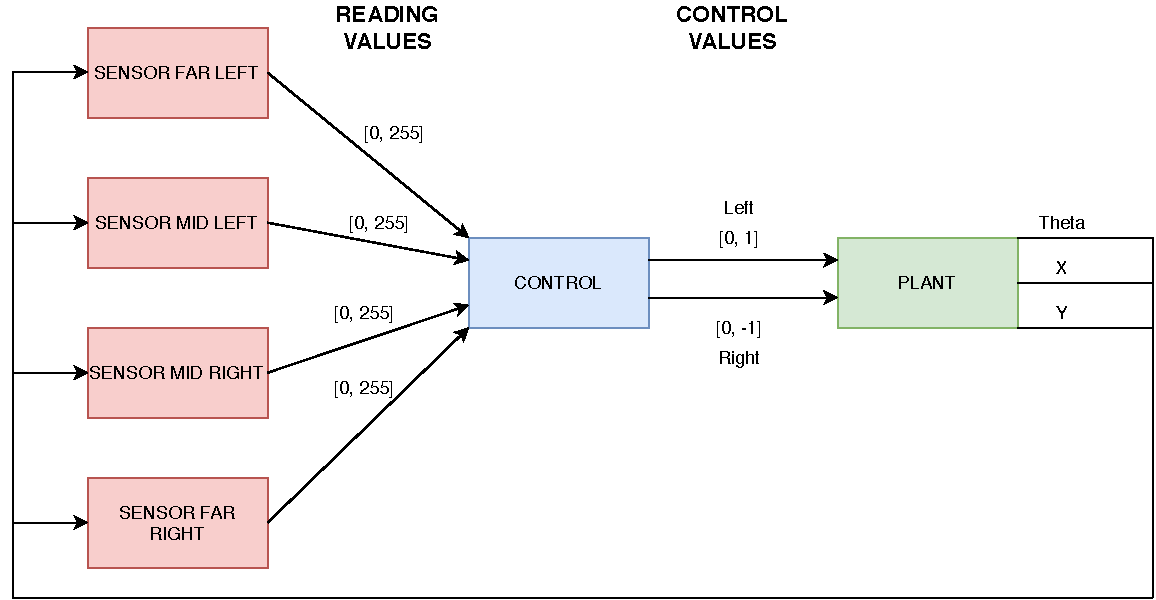
\includegraphics[width=\textwidth]{structure}
	\caption{Line follower robot structure}\label{fig:structure}
\end{figure}

\section{Controller}

The first step of our project is to implement a control algorithm for a
controller with four input sensors. In order to do so we have decided where the
sensors should be physically positioned on our Line Following Robot. In our
solution, the sensors are placed on the front side of the robot, lined up at one
centimeter of distance one from the other. Thus we have 2 left sensors, and 2
right sensor, in each one of these couple we have a far sensor, (the one nearer
to the side of the robot) and a mid sensor (the one near to the center of the
robot).

With this arrangement we have decided to use the four measures coming from the
sensors in the following way: we compute the average value of the two sensors on
the right and the average value of the two sensors on the left, in this way we
have two average values that can be used to decide the direction that our robot
should take.

These make possible to implement the control algorithm in an easier form,
improving also the resilience to possible erratic transient values.

\lstref{lst:control} shows the algorithm written in \code{misraC} code.

\lstinputlisting[language=C, label={lst:control}, caption={Control
algorithm.}]{controller.c}
